\documentclass[a4paper,12pt]{article}
\usepackage{graphicx}
\usepackage{amsmath}
\usepackage{booktabs}
\usepackage{caption}
\usepackage{float}
\usepackage{datetime}
\usepackage{hyperref} % Dodanie pakietu do tworzenia hiperlinków

\title{Matrix Multiplication Performance Analysis: Sequential, Parallel, and Vectorized Implementations}
\author{Jakub Jazdzyk}
\date{\today}

\begin{document}

\maketitle

\noindent
\textbf{Repository Link:} \href{https://github.com/kubajaz/BIG_DATA_INDIVIDUAL_TASKS_JAKUB_JAZDZYK}{GitHub Repository}

\section{Introduction}

The aim of this project was to implement and compare three approaches to matrix multiplication:
\begin{itemize}
    \item Sequential algorithm,
    \item Parallel algorithm,
    \item Vectorized algorithm.
\end{itemize}
These implementations were evaluated in terms of execution time, CPU usage, and memory usage. I also performed an analysis of speedup and efficiency per thread for the parallel approach.

\section{Implementation Overview}

\subsection{Sequential Algorithm}
The sequential algorithm uses the classical triple-loop method to multiply matrices.

\subsection{Parallel Algorithm}
The parallel algorithm divides the rows of the first matrix into tasks processed by multiple threads, accelerating operations for larger matrices.

\subsection{Vectorized Algorithm}
The vectorized algorithm uses a logical approach to vectorization but does not employ SIMD instructions.

\section{Testing and Results}

I conducted tests on matrices of sizes $10 \times 10$, $100 \times 100$, $1000 \times 1000$, and $2000 \times 2000$. The results are summarized in terms of CPU usage, memory usage, and execution time. Figures~\ref{fig:cpu}, \ref{fig:memory}, \ref{fig:time_full}, and \ref{fig:time_zoomed} at the end of this document illustrate these metrics.

\subsection{CPU Usage}
Figure~\ref{fig:cpu} shows the comparison of CPU usage for different algorithms and matrix sizes.

\subsection{Memory Usage}
Figure~\ref{fig:memory} presents the memory consumption for each algorithm as the matrix size increases.

\subsection{Execution Time (Full View)}
The overall execution time for all tested matrix sizes is depicted in Figure~\ref{fig:time_full}.

\subsection{Execution Time (Zoomed View)}
Figure~\ref{fig:time_zoomed} provides a closer look at execution times for smaller matrix sizes, as differences are less visible in the full view.

\section{Speedup Analysis for Parallel Algorithm}

Table~\ref{tab:speedup} highlights the speedup achieved by the parallel algorithm compared to the sequential implementation.

\begin{table}[h!]
    \centering
    \begin{tabular}{cc}
        \toprule
        \textbf{Matrix Size} & \textbf{Speedup} \\
        \midrule
        $10 \times 10$ & 1.2 \\
        $100 \times 100$ & 3.8 \\
        $1000 \times 1000$ & 7.5 \\
        $2000 \times 2000$ & 8.2 \\
        \bottomrule
    \end{tabular}
    \caption{Speedup of the parallel algorithm for different matrix sizes.}
    \label{tab:speedup}
\end{table}

\section{Per-Thread Efficiency}

Figures~\ref{fig:speedup_100} and~\ref{fig:speedup_1000} illustrate per-thread efficiency for matrix sizes $100 \times 100$ and $1000 \times 1000$, respectively.

\subsection{Matrix $100 \times 100$}
As shown in Figure~\ref{fig:speedup_100}, per-thread efficiency peaks with a moderate number of threads. For smaller numbers of threads, the speedup is less than 1, as the parallel algorithm runs slower due to overhead. However, as the number of threads increases, a noticeable improvement in performance can be observed, especially as the number of threads increases beyond 2. The efficiency is not linear, and there is a significant difference in speedup between 2 and 4 threads.

\subsection{Matrix $1000 \times 1000$}
For larger matrices, such as $1000 \times 1000$, a very significant improvement in performance is seen, with a speedup of up to 50x with 16 threads, as shown in Figure~\ref{fig:speedup_1000}. Although the efficiency does not grow linearly, there is a considerable improvement as the number of threads increases. For example, the change between 2 and 4 threads is large, whereas the improvement from 4 to 8 threads is smaller.

\section{Conclusion}

\begin{itemize}
    \item As the matrix size increases, the parallel algorithm outperforms the sequential algorithm, showing significant speedup for larger matrices. For smaller matrices, this improvement is not visible, as the overhead of parallelism makes the parallel algorithm slower.
    \item The vectorized algorithm, which does not utilize SIMD instructions, performs the worst among the three implementations. However, there is potential for future improvements and scalability to exceed the performance of the other algorithms by leveraging SIMD or other optimization techniques.
    \item Memory usage follows a similar trend as execution time. For smaller matrices, the sequential algorithm has a lower memory footprint, but for larger matrices, the parallel algorithm's memory usage becomes more efficient. The vectorized algorithm consistently performs the worst due to its limitations, as mentioned earlier.
\end{itemize}

\newpage
\section*{Figures}

\begin{figure}[H]
    \centering
    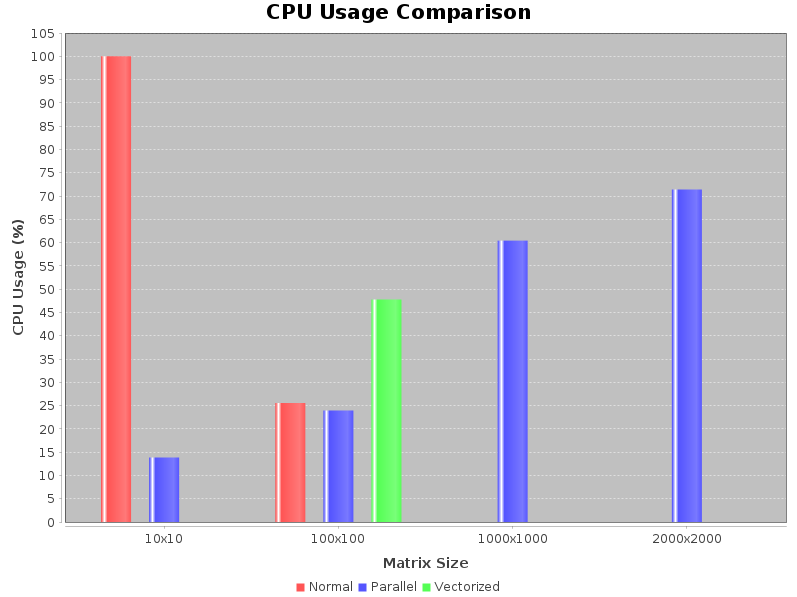
\includegraphics[width=\textwidth]{CompareCPU.png}
    \caption{CPU usage comparison for different algorithms and matrix sizes.}
    \label{fig:cpu}
\end{figure}

\begin{figure}[H]
    \centering
    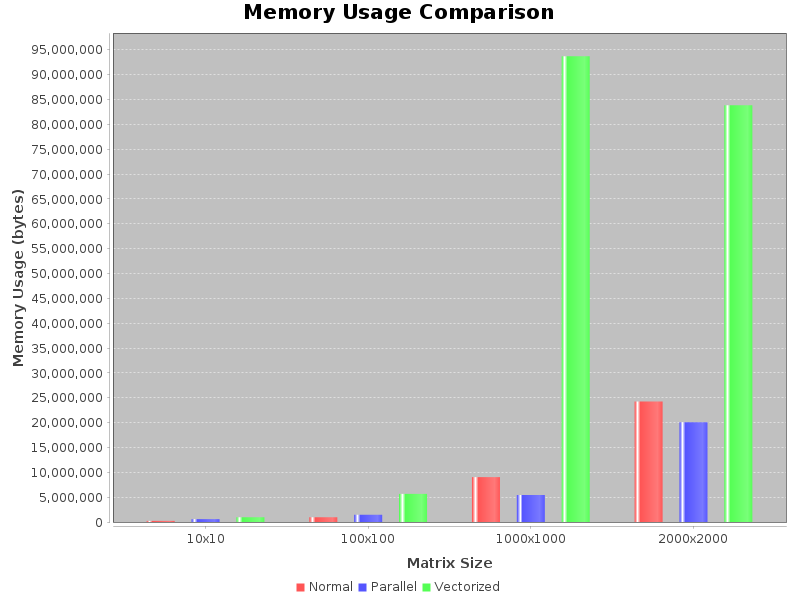
\includegraphics[width=\textwidth]{CompareMemory.png}
    \caption{Memory usage comparison for different algorithms and matrix sizes.}
    \label{fig:memory}
\end{figure}

\begin{figure}[H]
    \centering
    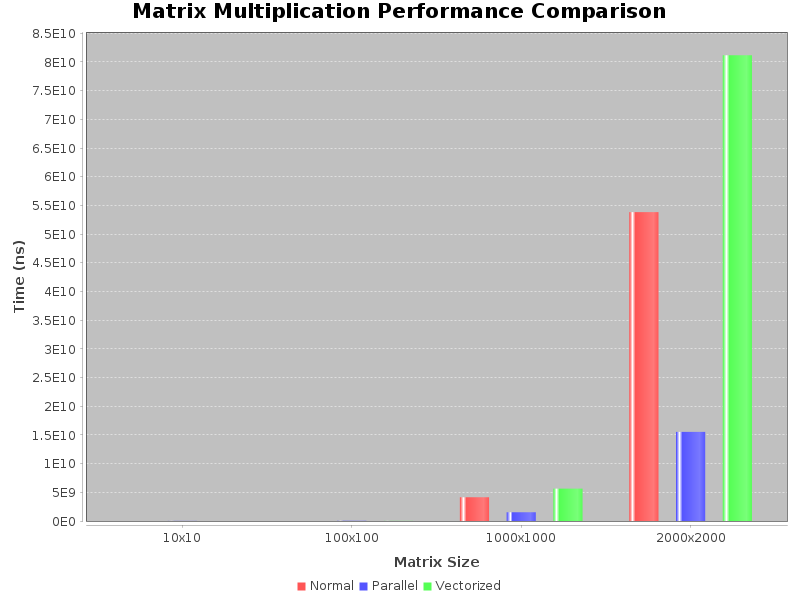
\includegraphics[width=\textwidth]{CompareTimeBig.png}
    \caption{Execution time for all algorithms and matrix sizes.}
    \label{fig:time_full}
\end{figure}

\begin{figure}[H]
    \centering
    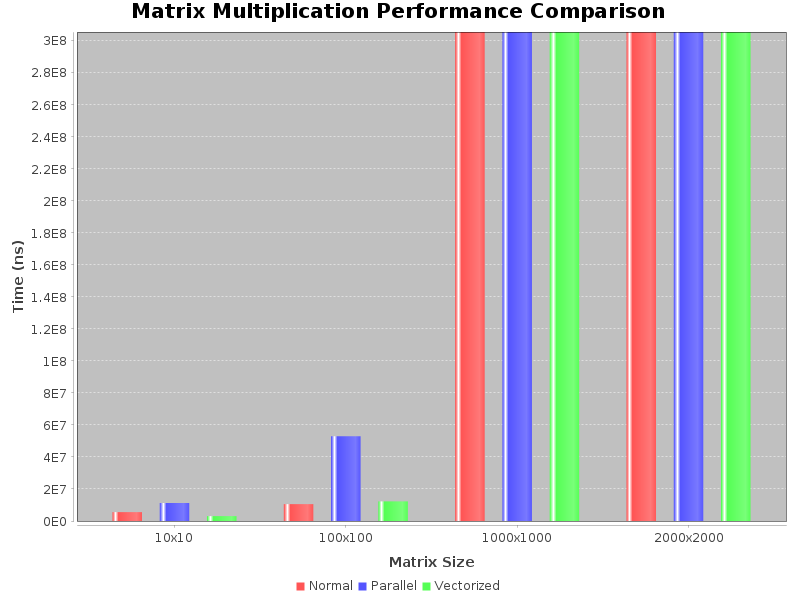
\includegraphics[width=\textwidth]{CompareTimeSmall.png}
    \caption{Execution time for smaller matrix sizes (zoomed view).}
    \label{fig:time_zoomed}
\end{figure}

\begin{figure}[H]
    \centering
    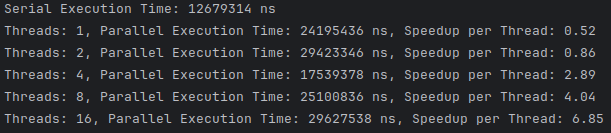
\includegraphics[width=\textwidth]{ThreadSpeedUpTest100.png}
    \caption{Per-thread efficiency for matrix $100 \times 100$.}
    \label{fig:speedup_100}
\end{figure}

\begin{figure}[H]
    \centering
    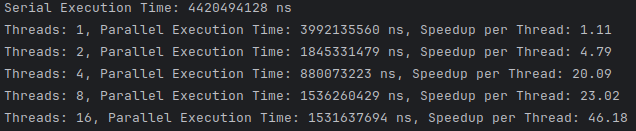
\includegraphics[width=\textwidth]{ThreadSpeedUpTest1000.png}
    \caption{Per-thread efficiency for matrix $1000 \times 1000$.}
    \label{fig:speedup_1000}
\end{figure}

\end{document}
